\subsection{Comparison}

At this moment, we have understood and tested both strategies, and it is moment to contrast each other and highlight their differences.

First of all we plot together the frequency histograms for the final wealth distribution for both models.

\begin{figure}[H]
    \centering
    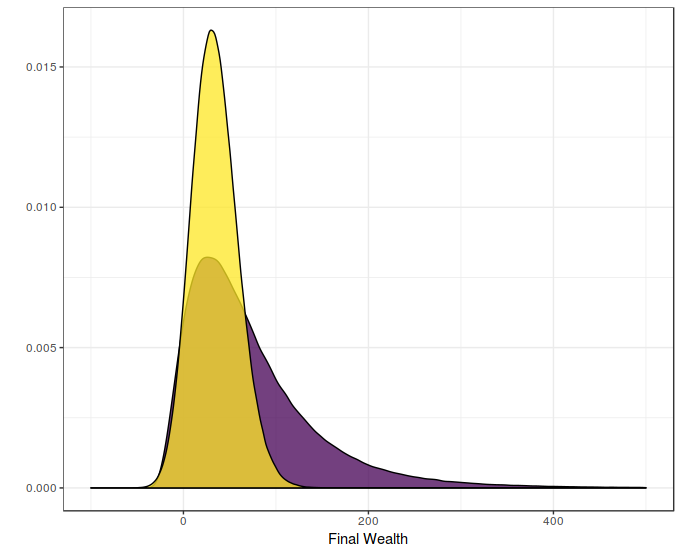
\includegraphics[scale=0.65]{./images/fw_both.png}
    \caption{Results of the simulation for the both models. Final wealth obtained for every simulation. The yellow one is the CPPI, and the purple one is the Alternative.}
    \label{fig:both_fw}
\end{figure}

Looking at Figure \ref{fig:both_fw} we may notice that they follow a considerably different distribution. We could say that the alternative model presents more dispersion, even though it is always a \textit{positive} deviation from the mean. 

In section \ref{sec:risk} we have discussed a little bit some implications of the definition of risk. Affirm that the alternative model presents more risk, just because its result is more disperse, would may seem a little simplistic. 

On the other hand, we can take a look at those rare cases when the final wealth happens to be negative. These are the cases worth exploring, for it is the scenario every investor is afraid of: losing money. Zooming in into the negative zone, as shown in figure \ref{fig:loss_both}, we can focus in the difference between the two models. Even though we can see some spurious differences in some places, the most honest answer is that it is not clear whose result is less risky.

\begin{figure}[H]
    \centering
    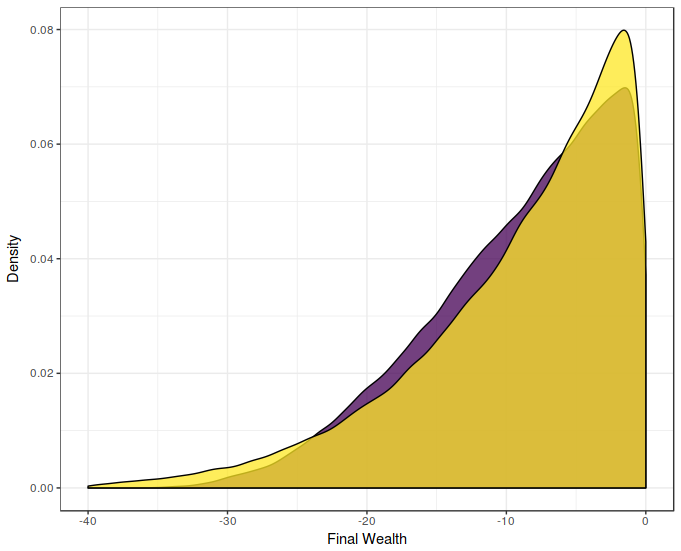
\includegraphics[scale=0.5]{./images/loss_both.png}
    \caption{Results of the simulation for the both models. Final wealth, filtered by negative values obtained for every simulation. The yellow one is the CPPI, and the purple one is the Alternative.}
    \label{fig:loss_both}
\end{figure}

In order to compare the degree of risk taken by every model, we make use of the \textit{Expected Shortfall}, as explained in section \ref{sec:risk}. If we set this parameter as the level of risk and we set it constant in both models, we can compare their returns. In~\cite{a:guillen-optimisation} it is shown that the Alternative model is able to set its Expected Shortfall (ES) by its $K$, using a closed formula.

Therefore, the approach is the following: We set a constant proportion $\pi$ for the CPPI model, we simulate it many times and measure the ES for the results. Then we find the $K$ in order to set the same ES on the Alternative model. This way we can simulate both models making sure they will assume the same risk, and thus we can freely compare their returns.

Setting $\alpha = 0.343$, $\sigma = 0.1544$, $a = 10$, $T = 60$, $A = 0.5$ and number of simulations $N = 100,000$ we find the results shown in table \ref{tab:cppi_alt}, in which we can see the outperformance of the alternative model, for many different levels of risk.

\begin{table}[H]
\centering
\caption{Results of $100,000$ simulations using different risk levels. These results match approximately those presented in \cite{a:guillen-optimisation}, on Table 1 at page 8. Any differences are attributable to the intrinsic randomness of simulations.}
\label{tab:cppi_alt}
\begin{tabular}{ccccccc}
\textbf{$\pi$} & \textbf{ES } & \textbf{$K$} & \textbf{CPPI ret} & \textbf{Alt ret} & \textbf{diff}  & \textbf{equiv $\pi$}\\
0.1   & -12.47  & 40.59  & 0.33     & 0.51    & 0.18    & 0.17\\
0.2   & -27.03  & 87.98  & 0.65     & 0.98    & 0.38    & 0.30 \\
0.3   & -42.99  & 139.95 & 0.95     & 1.42    & 0.46    & 0.45 \\
0.4   & -60.13  & 195.71 & 1.23     & 1.83    & 0.60    & 0.61 \\
0.5   & -78.25  & 255.02 & 1.5      & 2.22    & 0.71    & 0.69 \\
0.6   & -99.96  & 325.36 & 1.76     & 2.63    & 0.87    & 0.92 \\
0.7   & -120.61 & 392.56 & 2.00     & 3.00    & 1.00    & * \\
0.8   & -144.71 & 471.02 & 2.23     & 3.40    & 1.17    & * \\
0.9   & -172.94 & 562.92 & 2.39     & 3.81    & 1.42    & * \\
1     & -205.09 & 667.57 & 2.58     & 4.27    & 1.70    & *
\end{tabular}
\end{table}
